\scanpage{13}\mspage{12}
\deleted{\unsure{pr|pre}}inclure soit $\leq$, soit $\triangleleft$.

\deleted{b) $\leq$ et $\ll$ \unsure{déterminent} $\preccurlyeq$, car}
\[
\deleted{\unsure{G|F}\preccurlyeq F\Longleftrightarrow G\ll F}
\]

b) Chacune des relations $\leq$, $\ll$ détermine la relation $\parallel$. En effet
\[
\left\{\begin{aligned}
\text{a)}\quad F\parallel G &\ \deleted{\unsure{\Longleftrightarrow|\Longrightarrow}}\unsure{\Longrightarrow|\Longleftrightarrow}\
 \{F,G\}\ \text{majoré pour }\leq,\ \text{et }\mathop{\mathrm{Inf}}\limits_{\leq}(F,G)=\varnothing_F\\
\text{b)}\quad F\parallel G &\ \Longleftrightarrow\
 \deleted{\unsure{\mathrm{Inf}|\mathrm{S}}}\mathop{\mathrm{Sup}}\limits_{\ll}(F,G)\ \text{existe, et }\mathop{\mathrm{Inf}}\limits_{\ll} F,G=\varnothing_F
\end{aligned}\right.
\tag*{(1.24)}
\]
\margin{Verifier $\longrightarrow$}
(\uline{NB} $\varnothing_{\unsure{\mathcal{F}|\mathfrak{F}}}$ est à la fois plus petit \unsure{elémt|élémt|elément|élément} de $\mathcal{F}$ pour $\leq$, et pour $\ll$)

c) La relation $\ll$ détermine $\preccurlyeq$, par
\margin{$\times$}
\[
\begin{aligned}
F\preccurlyeq G &\Longleftrightarrow F\ll G,\ \text{et }\forall H\underset{\deleted{\unsure{\leq|<}}}{\in}\mathcal{F}\deleted{\unsure{K|H}}\ \text{on a}\\
&\hspace{2em}(H\parallel F\Longleftrightarrow H\parallel G)
\end{aligned}
\tag*{(1.25)}
\]
et on applique b).

d) La relation $\ll$ détermine $\mathcal{L}\subset\mathcal{F}$ comme l'ens des éléments minimaux de $\mathcal{F}\setminus\{\varnothing_{\mathcal{F}}\}$ :
\[
\mathcal{L}=\bigl\{\substack{X\in\mathcal{F}\\ X\neq\varnothing_{\mathcal{F}}}\mid
 Y\in\mathcal{F},\ Y\ll X,\ Y\neq\varnothing_{\unsure{\mathcal{F}|F|f}}\ \Rightarrow Y=X\bigr\} \tag*{(1.26)}
\]
(un \unsure{lieu|lien} est une \uline{figure} non vide dont le seul raffinement non vide est elle-$\overline{\mathrm m}$).

\deleted{Ceci dit $\ll$ implique la relation $\mathrel{\tikz[baseline=0pt,x=1em,y=1em]{\draw (-.38,.62)--(.38,.25)--(-.43,-.10); \draw (.34,.62)--(-.32,.25)--(.38,-.10);}}$ par}
\figure{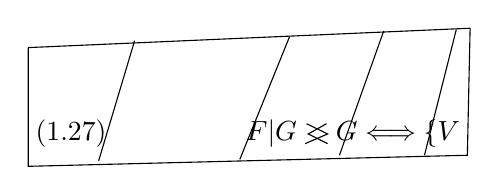
\begin{tikzpicture}[baseline=(trial.base),x=1em,y=1em]
\node[anchor=east,inner sep=0pt] (oldlabel) at (-5,0) {$\deleted{(1.27)}$};
\node[anchor=west,inner sep=0pt] (trial) at (0,0) {$\deleted{\unsure{F|G}\mathrel{\tikz[baseline=0pt,x=1em,y=1em]{\draw (-.38,.62)--(.38,.25)--(-.43,-.10); \draw (.34,.62)--(-.32,.25)--(.38,-.10);}} G\Longleftrightarrow\{V}$};
\draw ([xshift=-.25em,yshift=2.6em]oldlabel.north west) -- ([xshift=-.25em,yshift=-.65em]oldlabel.south west) -- ([xshift=.25em,yshift=-.25em]trial.south east) -- ([xshift=.35em,yshift=3.3em]trial.north east);
\draw ([xshift=-.25em,yshift=2.6em]oldlabel.north west) -- ([xshift=.35em,yshift=3.3em]trial.north east);
\draw ([xshift=-.3em,yshift=-.45em]oldlabel.south east) -- ([xshift=1.0em,yshift=2.85em]oldlabel.north east);
\draw ([xshift=-.2em,yshift=-.4em]trial.south west) -- ([xshift=1.6em,yshift=3em]trial.north west);
\draw ([xshift=3.4em,yshift=-.25em]trial.south west) -- ([xshift=5em,yshift=3.2em]trial.north west);
\draw ([xshift=-1.3em,yshift=-.25em]trial.south east) -- ([xshift=-.15em,yshift=3.25em]trial.north east);
\end{tikzpicture}}
% The old display label is inside the canceled drawing; its upper rule continues the strike through the preceding prose.
Je ne vois pas que $\ll$ ($+\ \preccurlyeq$, c'est kif-kif) détermine $\leq$, ni même $\mathrel{\tikz[baseline=0pt,x=1em,y=1em]{\draw (-.38,.62)--(.38,.25)--(-.43,-.10); \draw (.34,.62)--(-.32,.25)--(.38,-.10);}}$. Mais

\textcircled{\unsure{e|$\ominus$}}\quad $\ll$ et $\mathrel{\tikz[baseline=0pt,x=1em,y=1em]{\draw (-.38,.62)--(.38,.25)--(-.43,-.10); \draw (.34,.62)--(-.32,.25)--(.38,-.10);}}$ déterminent $\leq$ par
\margin{$\times$}
\[
G\leq F\quad\unsure{\Longleftarrow|\Longleftrightarrow}\quad (G\ll F\ \text{et}\ G\mathrel{\tikz[baseline=0pt,x=1em,y=1em]{\draw (-.38,.62)--(.38,.25)--(-.43,-.10); \draw (.34,.62)--(-.32,.25)--(.38,-.10);}} F) \tag*{(1.27)}
\]

Donc finalement,
